Die am häufigsten eingesetzte Kodiermethode im Kontext der Deflektometrie ist die Phasenkodierung.
Dieser Ansatz wird im Themengebiet der \glqq Phasenmessende Deflektometrie\grqq ~beschrieben.
Dabei verwendet man Streifenmuster die entlang der Ausbreitung der Streifen, den Grauwertverlauf einer trigonometrischen Funktion (z. B. Sinus- oder Kosinus-Funktion) annehmen.
Solche Muster nennt man auch sinusoidale Streifenmuster.
Die Szene bzw. der Monitor wird dabei über die Phase der Sinus-Funktion kodiert.
Das heißt, jeder Punkt auf einem Monitor, angegeben durch eine $x$- und eine $y$-Koordinate, wird durch eine Phase $\phi_x$ in $x$-Richtung und eine Phase $\phi_y$ in $y$-Richtung kodiert.
Verwendet man Streifenmuster, stellt man die Kodierung in zwei Bildern dar.
Das erste Bild kodiert die Spaltenpositionen durch die Phasen $\phi_x$ und das zweite Bild kodiert die Zeilenpositionen durch die Phasen $\phi_y$ (siehe Abbildung \ref{tikz:abbSinusoidaleStreifenmuster}).

\begin{figure}[H]
	\centering
		\begin{adjustbox}{width=\textwidth}
	\begin{tikzpicture}[every node/.style={inner sep=0,outer sep=0}]
	
		\node [anchor=north east] (imgSpalten) at (-0.03\textwidth,0) {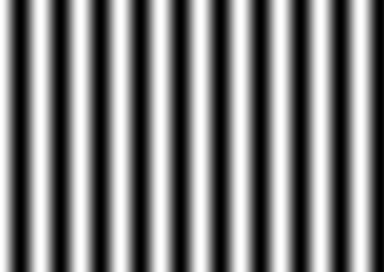
\includegraphics[frame,width=.47\textwidth]{02_grundlagenDerDeflektometrie/rekonstruktion/phasenKodierung/figures/sinusoidalesXMuster}};
		\node [below=0.2cm of imgSpalten, align = center] {Sinusoidales Muster zur Kodierung \\ der Spalten durch die Phasen $\phi_x$};
		\node [anchor=north west] (imgZeilen) at (0.03\textwidth,0) {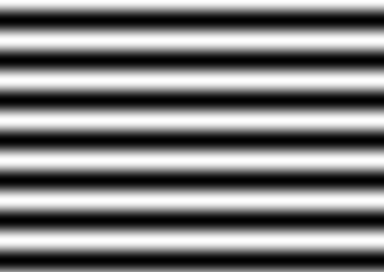
\includegraphics[frame,width=.47\textwidth]{02_grundlagenDerDeflektometrie/rekonstruktion/phasenKodierung/figures/sinusoidalesYMuster}};
		\node [below=0.2cm of imgZeilen, align = center] {Sinusoidales Muster zur Kodierung \\ der Zeilen durch die Phasen $\phi_y$};
		
	\end{tikzpicture}
\end{adjustbox}
\caption[Sinusoidale Streifenmuster]{Sinusoidale Streifenmuster zur Kodierung der Szene durch die Phasen $\left(\phi_x,\phi_y\right)$.}
		\label{tikz:abbSinusoidaleStreifenmuster}
\end{figure}

\noindent
Der Vorteil ist dabei die Kodierung durch die Grauwerte, die unabhängig von benachbarten Positionen dekodiert werden können.
Zur Dekodierung müssen aus den Grauwerten zunächst die Phasen bestimmt werden.
Dies funktioniert über ein sogenanntes Phasenschiebeverfahren \cite{carre}, bei dem weitere Bildaufnahmen mit Phasenverschiebungen der trigonometrischen Funktion vorgenommen werden.
Durch die Periodizität der verwendeten trigonometrischen Funktion sind die bestimmten Phasen zunächst noch relativ zu den einzelnen Perioden angegeben.
In einem weiteren Schritt muss eine sogenannte Phasenentfaltung bzw. ein \glqq Phase Unwrap\grqq ~durchgeführt werden (siehe auch Definition \ref{def:phasenentfaltung}), damit die absoluten Phasen $\left(\phi_x,\phi_y\right)$ bestimmt werden können.
Die Dekodierung über das \glqq Phase Unwrap\grqq ~erfolgt dabei durch die Verwendung von weiteren sinusoidalen Streifenmustern mit unterschiedlicher Frequenz.
Diese Art der Kodierung erfordert deshalb weitere Bilder.
Ein solches Verfahren wird im Kapitel \ref{sec:bestimmungDeflektometrischeRegistrierung} genauer beschrieben.

\p
Es sind damit zunächst mehrere Bildaufnahmen erforderlich.
Da solche Verfahren damit mehr Ressourcen verwenden, fokussieren sich einige Forschungsarbeiten darauf, die Anzahl der benötigten Muster zu reduzieren.
Der heutige technische Stand ermöglicht es bereits z. B. durch Überlagerung von Mustern und weiteren Optimierungen, die Phasendekodierung durch eine einzige Kameraaufnahme umzusetzen (vgl. \cite{waveletPMD}).
Allerdings wird dadurch mehr Information kodiert auf gleichem Ort, wodurch Unschärfen und starke Krümmungen des Objekts das Ergebnis der deflektometrischen Messung stärker verfälschen können.